\chapter{Practical details}



\section{Cross-correlation levels against recording length}
\begin{figure}[H]
    \centering
    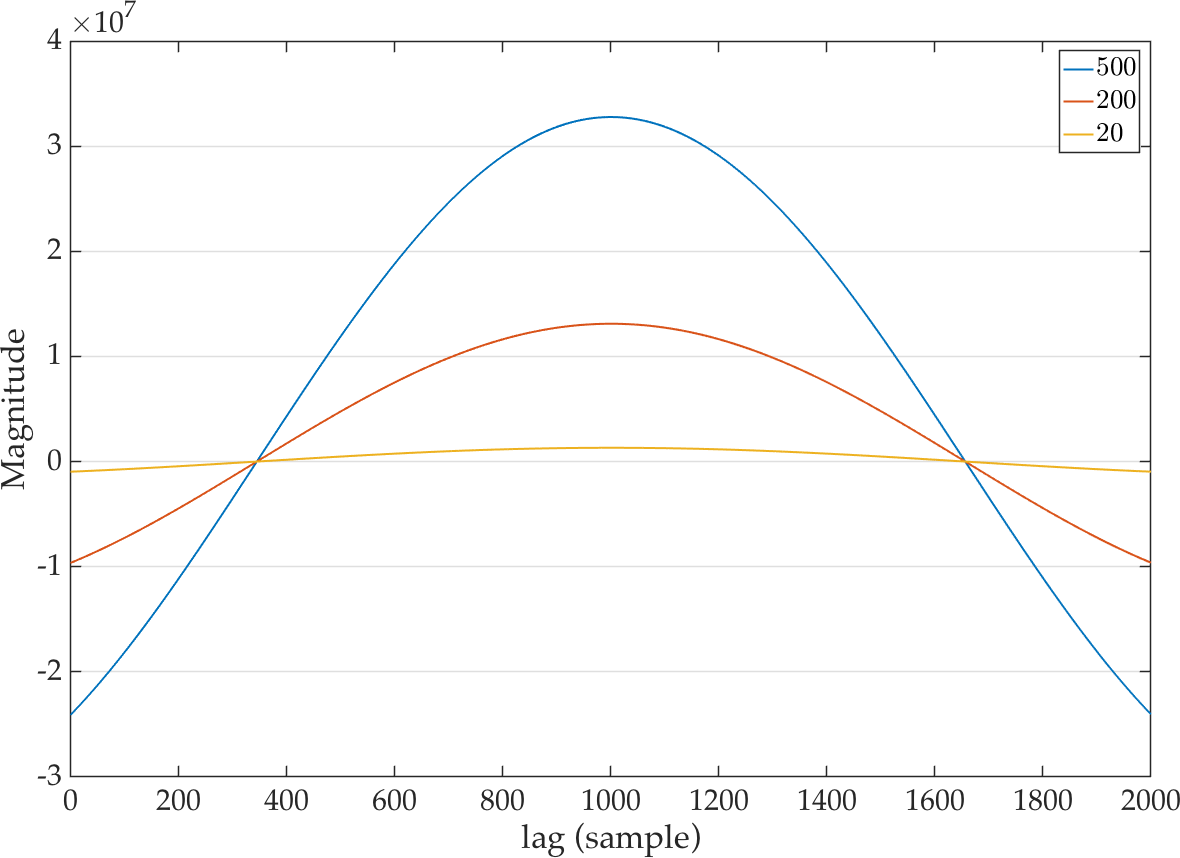
\includegraphics[width=0.8\textwidth]{Figures/20200500.png}
    \caption{Magnitude of the cross-correlation of a pair of microphones. No additive noise. The blue line is the magnitude of the cross correlation with PHAT weighting for a 50Hz sin wave with different recording time 500s (blue), 200s (orange) and 20s (orange)}
    \label{fig:xcorr20500hz}
\end{figure}

\section{Field of view calculation}
\begin{figure}[H]
    \centering
    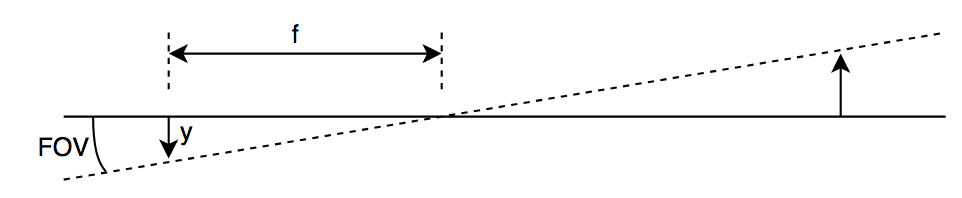
\includegraphics[width=0.8\textwidth]{Figures/FOV.png}
    \caption{Field of view}
    \label{fig:fov}
\end{figure}
In order to overlap the map to the picture, the field of view (FOV) is calculated.
\begin{equation}
    FOV = 2 * arctan(\frac{y}{f})
\end{equation}
with f the focal length of the lens and y the height or width of the sensor. In some camera, there is a crop factor which need to be multiply to y. In the case of the FUJIFILM xt-20, the crop factor is 1.5 and sensor dimensions is $23.5*15.6$mm. For a focal length of $16mm$ The horizontal FOV is $44\degree$ and the vertical FOV is $33\degree$. Therefore the horizontal span is $88\degree$ and the vertical span is $66\degree$

\section{Generation of white noise}

\section{Generation of pink noise}

\section{Simulating a tetrahedral array}

\section{Other system diagram}


\section{Microphone information}\label{app:micLocs}
The sensitivities of the microphones used for the tetrahedral array are tabulated below. These sensitivities are only relevant for the outdoor measurements. For simulations all microphones are assumed to have equal sensitivity.
\begin{table}[H]
\centering
    \begin{tabular}{ll} \toprule
	{Mic}	&	{Sensitivity}\\
	    \bottomrule 
	    $M_1$   &   6.694 mV/Pa                   \\
	    $M_2$   &   5.863 mV/Pa                   \\
	    $M_3$   &   5.743 mV/Pa                   \\
		$M_4$   &   5.696 mV/Pa                   \\
		\bottomrule 
	\end{tabular}
\end{table}
The tetrahedral array was used with two different apertures, 1m and 39.5cm, resulting in two different array configurations, large and small. The (x,y,z) placement of the 4 microphones for the configurations are given below. The origin of the coordinate system signifies the viewpoint of the array, i.e, the (azimuth,elevation) shown in the results are relative to the origin on these co-ordinates.
For the large aperture,
\begin{table}[H]
\centering
    \begin{tabular}{ll} \toprule
	{Mic}	&	{Position (m)}\\
	    \bottomrule 
     $M_1$   &   (0.5, 0, 0) \\
     $M_2$   &   (-0.5, 0, 0) \\
     $M_3$   &   (0, -0.866, 0) \\
     $M_4$   &   (0, -0.433, 0.7071) \\
	\bottomrule 
	\end{tabular}
\end{table}

And for the small aperture,
\begin{table}[H]
\centering
    \begin{tabular}{ll} \toprule
	{Mic}	&	{Position (m)}\\
	    \bottomrule 
     $M_1$   &   (0.1975, 0, 0) \\
     $M_2$   &   (-0.1975, 0, 0)\\
     $M_3$   &   (0, -0.3421, 0)\\
     $M_4$   &   (0, -0.171, 0.2793) \\	\bottomrule 
	\end{tabular}
\end{table}
For simulations where less than 4 microphones are used, the microphone used are
\begin{itemize}
    \item 2 Microphones: Only $M_1$ and $M_2$
    \item 3 Microphones: $M_1$, $M_2$ and $M_3$
\end{itemize}